\documentclass[xcolor=svgnames]{beamer}
\usepackage[utf8]{inputenc}
\usepackage[T1]{fontenc} % Added for better font encoding
\usepackage{xcolor}
\usepackage{booktabs} % for tables if needed
\usepackage{amsmath} % for math
\usepackage{graphicx} % For images if needed
\usepackage{hyperref} % For links
\usetheme{Madrid}

% COLORS (As provided)
\definecolor{mqred}{RGB}{166, 25, 46}
\definecolor{mqdeepred}{RGB}{118, 35, 47}
\definecolor{mqgray}{RGB}{55, 58, 54}
\definecolor{mqlightgray}{RGB}{237, 235, 229}
\definecolor{mqmagenta}{RGB}{198, 0, 126}
\usecolortheme[named=mqred]{structure}
\setbeamercolor{title in head/foot}{bg=mqlightgray, fg=mqgray}
\setbeamercolor{author in head/foot}{bg=mqdeepred}
\setbeamercolor{page number in head/foot}{bg=mqdeepred, fg=mqlightgray}

% FOOTNOTE ARRANGEMENTS (As provided)
\makeatletter
\setbeamertemplate{footline}{
  \leavevmode%
  \hbox{%
  \begin{beamercolorbox}[wd=.5\paperwidth,ht=2.25ex,dp=1ex,center]{author in head/foot}%
    \usebeamerfont{author in head/foot}\insertshortauthor\expandafter\ifblank\expandafter{\beamer@shortinstitute}{}{~~(\insertshortinstitute)}
  \end{beamercolorbox}%
  \begin{beamercolorbox}[wd=.4\paperwidth,ht=2.25ex,dp=1ex,center]{title in head/foot}%
    \usebeamerfont{title in head/foot}\insertshorttitle
  \end{beamercolorbox}%
  \begin{beamercolorbox}[wd=.1\paperwidth,ht=2.25ex,dp=1ex,center]{page number in head/foot}%
    \usebeamerfont{page number in head/foot}\insertframenumber{} / \inserttotalframenumber
  \end{beamercolorbox}}%
  \vskip0pt%
}
\makeatother
\beamertemplatenavigationsymbolsempty

% TITLE, AUTHORS, INSTITUTE, DATE
\title[Thermo: Particles \& Energy]{Thermodynamics Lesson 1: Particles, Temperature \& Energy Flow}
\author[P. Haynes]{Mr Haynes}
\institute[GHS]{Gosford High School}
\date{\today} % Or specific date

% LOGO (Optional)
%\titlegraphic{\includegraphics[height=2.5cm]{logo.jpg}} % Change the logo path as needed

\begin{document}

\begin{frame}
    \titlepage
\end{frame}

\begin{frame}{Outline}
    \tableofcontents
\end{frame}

\section{Introduction}
\begin{frame}{What is Thermodynamics?}
    \frametitle{Introduction: Why Study Thermodynamics?}
    \textbf{Focus Inquiry Question 1:} How are temperature, thermal energy, and particle motion related?
    \vspace{1em}

    \begin{itemize}
        \item \textbf{Definition:} The study of energy, its transfer (heat, work), and transformations.
        \item \textbf{Think/Pair/Share:} Why does a metal chair feel colder than a wooden one at the same room temperature?
        \vspace{1em}
        \item \textbf{Relevance:}
        \begin{itemize}
            \item \textit{Historical:} Driven by the need to understand and improve Steam Engines (Industrial Revolution).
            \item \textit{Future:} Crucial for Climate Science (energy efficiency), Sustainable Technologies, Computing (heat limits).
        \end{itemize}
        \item \textbf{Key Terms (Worksheet 1):}
        \begin{itemize}
            \item Temperature (Measure of \textit{average} particle Kinetic Energy - KE) [N1]
            \item Thermal Energy (Total internal energy - KE + Potential Energy) [N1]
            \item Heat (Transfer of thermal energy due to temperature difference)
        \end{itemize}
    \end{itemize}
\end{frame}

\section{Particle Model and Temperature}
\begin{frame}{Particles in Motion [N1]}
    \frametitle{Temperature and Particle Kinetic Energy}
    \begin{itemize}
        \item Matter is made of particles (atoms/molecules) constantly in motion.
        \item Temperature is directly related to the \textit{average} kinetic energy of these particles.
        \item Higher Temperature $\implies$ Higher Average KE $\implies$ Faster Particle Motion (vibration, translation, rotation).
        \item Lower Temperature $\implies$ Lower Average KE $\implies$ Slower Particle Motion.
    \end{itemize}
    \vspace{1em}
    \textbf{Visualisation:} PhET Simulation "Energy Forms and Changes" shows this link.
    % Placeholder for a screenshot or diagram
    \begin{center}
    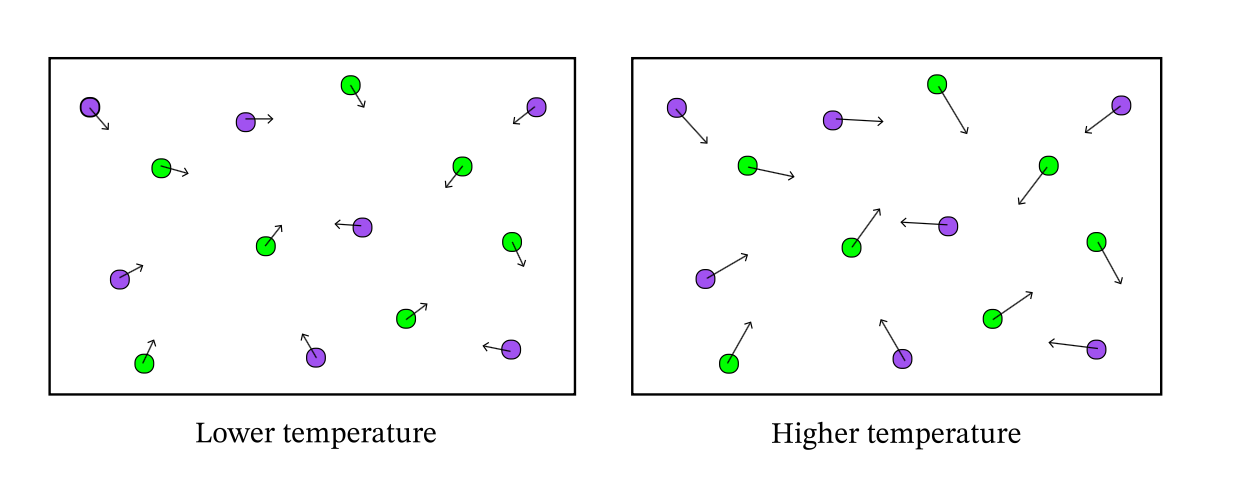
\includegraphics[width=0.6\textwidth]{placeholder_phet_particles.png} % Replace with actual image
    \end{center}
    Observe particle speed increasing as heat is added.
\end{frame}

\section{Heat Transfer Mechanisms}
\begin{frame}{How Does Heat Move? [N4]}
    \frametitle{Mechanisms of Heat Transfer}
    Heat (thermal energy) transfers via three main mechanisms:
    \vspace{1em}

    \begin{columns}[T] % Align tops
        \begin{column}{0.33\textwidth}
            \textbf{1. Conduction}
            \begin{itemize}
                \item Transfer through direct particle collisions.
                \item Dominant in solids.
                \item Faster in materials with closely packed particles / free electrons (e.g., metals).
                \item \textit{Example:} Hot spoon handle.
            \end{itemize}
        \end{column}
        \begin{column}{0.33\textwidth}
            \textbf{2. Convection}
            \begin{itemize}
                \item Transfer by the movement of fluids (liquids/gases).
                \item Hotter fluid is less dense and rises; cooler fluid sinks. Creates currents.
                \item \textit{Example:} Boiling water, sea breeze.
            \end{itemize}
        \end{column}
        \begin{column}{0.33\textwidth}
            \textbf{3. Radiation}
            \begin{itemize}
                \item Transfer via electromagnetic waves (infrared).
                \item Requires NO medium.
                \item All objects above absolute zero radiate.
                \item \textit{Example:} Heat from sun, warmth from a fire.
            \end{itemize}
        \end{column}
    \end{columns}
    \vspace{1em}
    \textit{Activity 1 provides demonstrations/simulations for these.}
\end{frame}

\section{Thermal Equilibrium Intro}
\begin{frame}{Reaching a Balance [N2 Intro]}
    \frametitle{Thermal Equilibrium}
    \begin{itemize}
        \item \textbf{Direction of Flow (Inquiry Q3 link):} Heat naturally flows from a hotter object to a colder object when they are in thermal contact.
        \item \textbf{Equilibrium Definition:} The state reached when there is \textbf{no net flow} of heat between objects in thermal contact.
        \item \textbf{Condition:} This occurs when the objects reach the \textbf{same temperature}.
        \item \textit{Example:} A cold drink eventually warms up to room temperature. The drink and the room air reach thermal equilibrium.
    \end{itemize}
    \begin{center}
    % Placeholder for diagram: Hot block -> Cold block = Heat Flow Arrow
    \fbox{\includegraphics[width=0.5\textwidth]{placeholder_equilibrium.png}} % Replace
    \end{center}
\end{frame}

\section{Summary}
\begin{frame}{Lesson 1 Summary}
    \begin{itemize}
        \item Thermodynamics studies energy transfer and transformation.
        \item Temperature reflects average particle kinetic energy [N1].
        \item Heat is energy transferred due to temperature differences.
        \item Heat transfers via Conduction, Convection, Radiation [N4].
        \item Thermal Equilibrium is reached when temperatures are equal (no net heat flow) [N2].
    \end{itemize}
    \vspace{1em}
    \textbf{Next Steps:}
    \begin{itemize}
        \item Complete Worksheet 1 (Definitions, Explanations).
        \item Complete \#MarkSense Quiz 1 (Check understanding).
        \item Preview Lesson 2: Quantifying heat transfer (Calculations!).
    \end{itemize}
\end{frame}

\begin{frame}
    \centering
    \textbf{Thank you!}\\
    Questions?
\end{frame}

\end{document}
